% Options for packages loaded elsewhere
\PassOptionsToPackage{unicode}{hyperref}
\PassOptionsToPackage{hyphens}{url}
%
\documentclass[
]{article}
\usepackage{amsmath,amssymb}
\usepackage{lmodern}
\usepackage{iftex}
\ifPDFTeX
  \usepackage[T1]{fontenc}
  \usepackage[utf8]{inputenc}
  \usepackage{textcomp} % provide euro and other symbols
\else % if luatex or xetex
  \usepackage{unicode-math}
  \defaultfontfeatures{Scale=MatchLowercase}
  \defaultfontfeatures[\rmfamily]{Ligatures=TeX,Scale=1}
\fi
% Use upquote if available, for straight quotes in verbatim environments
\IfFileExists{upquote.sty}{\usepackage{upquote}}{}
\IfFileExists{microtype.sty}{% use microtype if available
  \usepackage[]{microtype}
  \UseMicrotypeSet[protrusion]{basicmath} % disable protrusion for tt fonts
}{}
\makeatletter
\@ifundefined{KOMAClassName}{% if non-KOMA class
  \IfFileExists{parskip.sty}{%
    \usepackage{parskip}
  }{% else
    \setlength{\parindent}{0pt}
    \setlength{\parskip}{6pt plus 2pt minus 1pt}}
}{% if KOMA class
  \KOMAoptions{parskip=half}}
\makeatother
\usepackage{xcolor}
\usepackage[margin=1in]{geometry}
\usepackage{color}
\usepackage{fancyvrb}
\newcommand{\VerbBar}{|}
\newcommand{\VERB}{\Verb[commandchars=\\\{\}]}
\DefineVerbatimEnvironment{Highlighting}{Verbatim}{commandchars=\\\{\}}
% Add ',fontsize=\small' for more characters per line
\usepackage{framed}
\definecolor{shadecolor}{RGB}{248,248,248}
\newenvironment{Shaded}{\begin{snugshade}}{\end{snugshade}}
\newcommand{\AlertTok}[1]{\textcolor[rgb]{0.94,0.16,0.16}{#1}}
\newcommand{\AnnotationTok}[1]{\textcolor[rgb]{0.56,0.35,0.01}{\textbf{\textit{#1}}}}
\newcommand{\AttributeTok}[1]{\textcolor[rgb]{0.77,0.63,0.00}{#1}}
\newcommand{\BaseNTok}[1]{\textcolor[rgb]{0.00,0.00,0.81}{#1}}
\newcommand{\BuiltInTok}[1]{#1}
\newcommand{\CharTok}[1]{\textcolor[rgb]{0.31,0.60,0.02}{#1}}
\newcommand{\CommentTok}[1]{\textcolor[rgb]{0.56,0.35,0.01}{\textit{#1}}}
\newcommand{\CommentVarTok}[1]{\textcolor[rgb]{0.56,0.35,0.01}{\textbf{\textit{#1}}}}
\newcommand{\ConstantTok}[1]{\textcolor[rgb]{0.00,0.00,0.00}{#1}}
\newcommand{\ControlFlowTok}[1]{\textcolor[rgb]{0.13,0.29,0.53}{\textbf{#1}}}
\newcommand{\DataTypeTok}[1]{\textcolor[rgb]{0.13,0.29,0.53}{#1}}
\newcommand{\DecValTok}[1]{\textcolor[rgb]{0.00,0.00,0.81}{#1}}
\newcommand{\DocumentationTok}[1]{\textcolor[rgb]{0.56,0.35,0.01}{\textbf{\textit{#1}}}}
\newcommand{\ErrorTok}[1]{\textcolor[rgb]{0.64,0.00,0.00}{\textbf{#1}}}
\newcommand{\ExtensionTok}[1]{#1}
\newcommand{\FloatTok}[1]{\textcolor[rgb]{0.00,0.00,0.81}{#1}}
\newcommand{\FunctionTok}[1]{\textcolor[rgb]{0.00,0.00,0.00}{#1}}
\newcommand{\ImportTok}[1]{#1}
\newcommand{\InformationTok}[1]{\textcolor[rgb]{0.56,0.35,0.01}{\textbf{\textit{#1}}}}
\newcommand{\KeywordTok}[1]{\textcolor[rgb]{0.13,0.29,0.53}{\textbf{#1}}}
\newcommand{\NormalTok}[1]{#1}
\newcommand{\OperatorTok}[1]{\textcolor[rgb]{0.81,0.36,0.00}{\textbf{#1}}}
\newcommand{\OtherTok}[1]{\textcolor[rgb]{0.56,0.35,0.01}{#1}}
\newcommand{\PreprocessorTok}[1]{\textcolor[rgb]{0.56,0.35,0.01}{\textit{#1}}}
\newcommand{\RegionMarkerTok}[1]{#1}
\newcommand{\SpecialCharTok}[1]{\textcolor[rgb]{0.00,0.00,0.00}{#1}}
\newcommand{\SpecialStringTok}[1]{\textcolor[rgb]{0.31,0.60,0.02}{#1}}
\newcommand{\StringTok}[1]{\textcolor[rgb]{0.31,0.60,0.02}{#1}}
\newcommand{\VariableTok}[1]{\textcolor[rgb]{0.00,0.00,0.00}{#1}}
\newcommand{\VerbatimStringTok}[1]{\textcolor[rgb]{0.31,0.60,0.02}{#1}}
\newcommand{\WarningTok}[1]{\textcolor[rgb]{0.56,0.35,0.01}{\textbf{\textit{#1}}}}
\usepackage{longtable,booktabs,array}
\usepackage{calc} % for calculating minipage widths
% Correct order of tables after \paragraph or \subparagraph
\usepackage{etoolbox}
\makeatletter
\patchcmd\longtable{\par}{\if@noskipsec\mbox{}\fi\par}{}{}
\makeatother
% Allow footnotes in longtable head/foot
\IfFileExists{footnotehyper.sty}{\usepackage{footnotehyper}}{\usepackage{footnote}}
\makesavenoteenv{longtable}
\usepackage{graphicx}
\makeatletter
\def\maxwidth{\ifdim\Gin@nat@width>\linewidth\linewidth\else\Gin@nat@width\fi}
\def\maxheight{\ifdim\Gin@nat@height>\textheight\textheight\else\Gin@nat@height\fi}
\makeatother
% Scale images if necessary, so that they will not overflow the page
% margins by default, and it is still possible to overwrite the defaults
% using explicit options in \includegraphics[width, height, ...]{}
\setkeys{Gin}{width=\maxwidth,height=\maxheight,keepaspectratio}
% Set default figure placement to htbp
\makeatletter
\def\fps@figure{htbp}
\makeatother
\setlength{\emergencystretch}{3em} % prevent overfull lines
\providecommand{\tightlist}{%
  \setlength{\itemsep}{0pt}\setlength{\parskip}{0pt}}
\setcounter{secnumdepth}{-\maxdimen} % remove section numbering
\ifLuaTeX
  \usepackage{selnolig}  % disable illegal ligatures
\fi
\IfFileExists{bookmark.sty}{\usepackage{bookmark}}{\usepackage{hyperref}}
\IfFileExists{xurl.sty}{\usepackage{xurl}}{} % add URL line breaks if available
\urlstyle{same} % disable monospaced font for URLs
\hypersetup{
  pdftitle={Computer assignment 3: DNA Sequence Analysis},
  pdfauthor={BIOS 11141 - Computational Biology},
  hidelinks,
  pdfcreator={LaTeX via pandoc}}

\title{Computer assignment 3: DNA Sequence Analysis}
\author{BIOS 11141 - Computational Biology}
\date{}

\begin{document}
\maketitle

\textbf{Assignment objectives:} 1. Learn about NCBI sequence databases
2. Write a function to find Open Reading Frames (ORFs) of a given DNA
sequence 3. Find the origion of replication (\emph{oriC}) of a given DNA
molecule \span

For your work in this assignment, please add your answers to the file
entitled `Ans3\_LastnameFirstname.Rmd' and change the file name to have
\emph{your actual} first and last name. The answers are formatted to be
in blue and all questions are in green, in both this document and in the
answers document. Upload your answers file as an .Rmd and .html to
Canvas by 2:30 p.m. the Friday of next week. \span  

This week's assignment has been adopted from A Little Book of R for
Bioinformatics, written by Avril Coghlan; Dr.~Kondrashov's labs from
2015's BIOS 10602; and Bioinformatics Algorithms An Active Learning
Approach book, written by Phillip Compeau \& Pavel Pevzner. \span  

R can be a powerful tool to carry out analyses common in bioinformatics.
Some well known bioinformatics scripts for R are the
\href{http://www.bioconductor.org}{Bioconductor} set of R packages that
contain several functions for analyzing biological data sets such as
microarray data; and the
\href{https://cran.r-project.org/web/packages/seqinr/index.html}{SeqinR}
package that contain R functions for obtaining sequences from DNA and
protein databases, and for analyzing DNA and protein sequences.

For this assignment we're going to focus on computational analysis of
biological sequence data such as genome sequences. Many authors have
written specialized packages for R that don't come with the standard R
installation. We need to install and load the SeqinR package before we
can use it. Execute the commands:

\begin{Shaded}
\begin{Highlighting}[]
\FunctionTok{install.packages}\NormalTok{(}\StringTok{\textquotesingle{}seqinr\textquotesingle{}}\NormalTok{, }\AttributeTok{repos=}\StringTok{\textquotesingle{}http://cran.us.r{-}project.org\textquotesingle{}}\NormalTok{)}
\end{Highlighting}
\end{Shaded}

\begin{verbatim}
## Installing package into 'C:/Users/icthy/AppData/Local/R/win-library/4.2'
## (as 'lib' is unspecified)
\end{verbatim}

\begin{verbatim}
## package 'seqinr' successfully unpacked and MD5 sums checked
## 
## The downloaded binary packages are in
##  C:\Users\icthy\AppData\Local\Temp\RtmpicxFC0\downloaded_packages
\end{verbatim}

\begin{Shaded}
\begin{Highlighting}[]
\CommentTok{\#use either "library("seqinr")" or "require("seqinr")" to load the newly installed package onto R.}
\end{Highlighting}
\end{Shaded}

\hypertarget{part-1-the-ncbi-sequence-database}{%
\subsection{Part 1: The NCBI Sequence
Database}\label{part-1-the-ncbi-sequence-database}}

The National Center for Biotechnology Information (NCBI) maintains a
huge database of all the DNA and protein sequence data that has been
collected. Each sequence in the NCBI database is stored in a separate
record and is assigned a unique identifier called an \textbf{accession
number} that can be used to refer to that sequence record. You can
easily retrieve DNA or protein sequence data from the NCBI Sequence
Database via its website: \url{www.ncbi.nlm.nih.gov}. The NCBI accession
code for severe acute respiratory symdrome coronavirus 2 (SARS-CoV-2) is
NC\_045512.2. Go to the NCBI website, type ``NC\_045512.2'' in the
search box, and press the ``Search'' button.

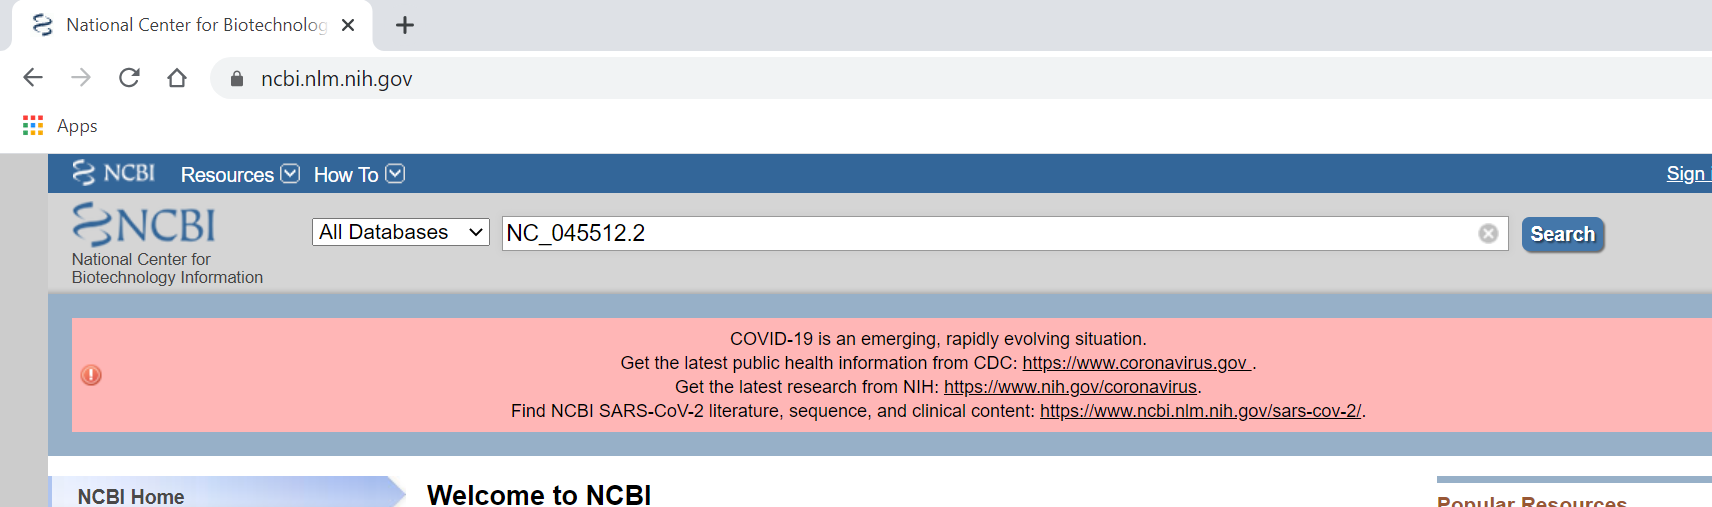
\includegraphics{./Images/img1.png}

There are many databases on the NCBI website. On the results page you
will see the number of hits for ``NC\_045512.2'' in each of the NCBI
databases on the NCBI website. \textbf{For example, the PubMed database
contains abstracts from scientific papers, the Nucleotide database
contains DNA and RNA sequence data, the Protein database contains
protein sequence data, and so on. We are looking for the RNA genome
sequence of SARS-CoV-2, so click on the Nucleotide database.}

When you click on the icon for the NCBI Nucleotide database, it will
bring you to the record for NC\_045512.2:

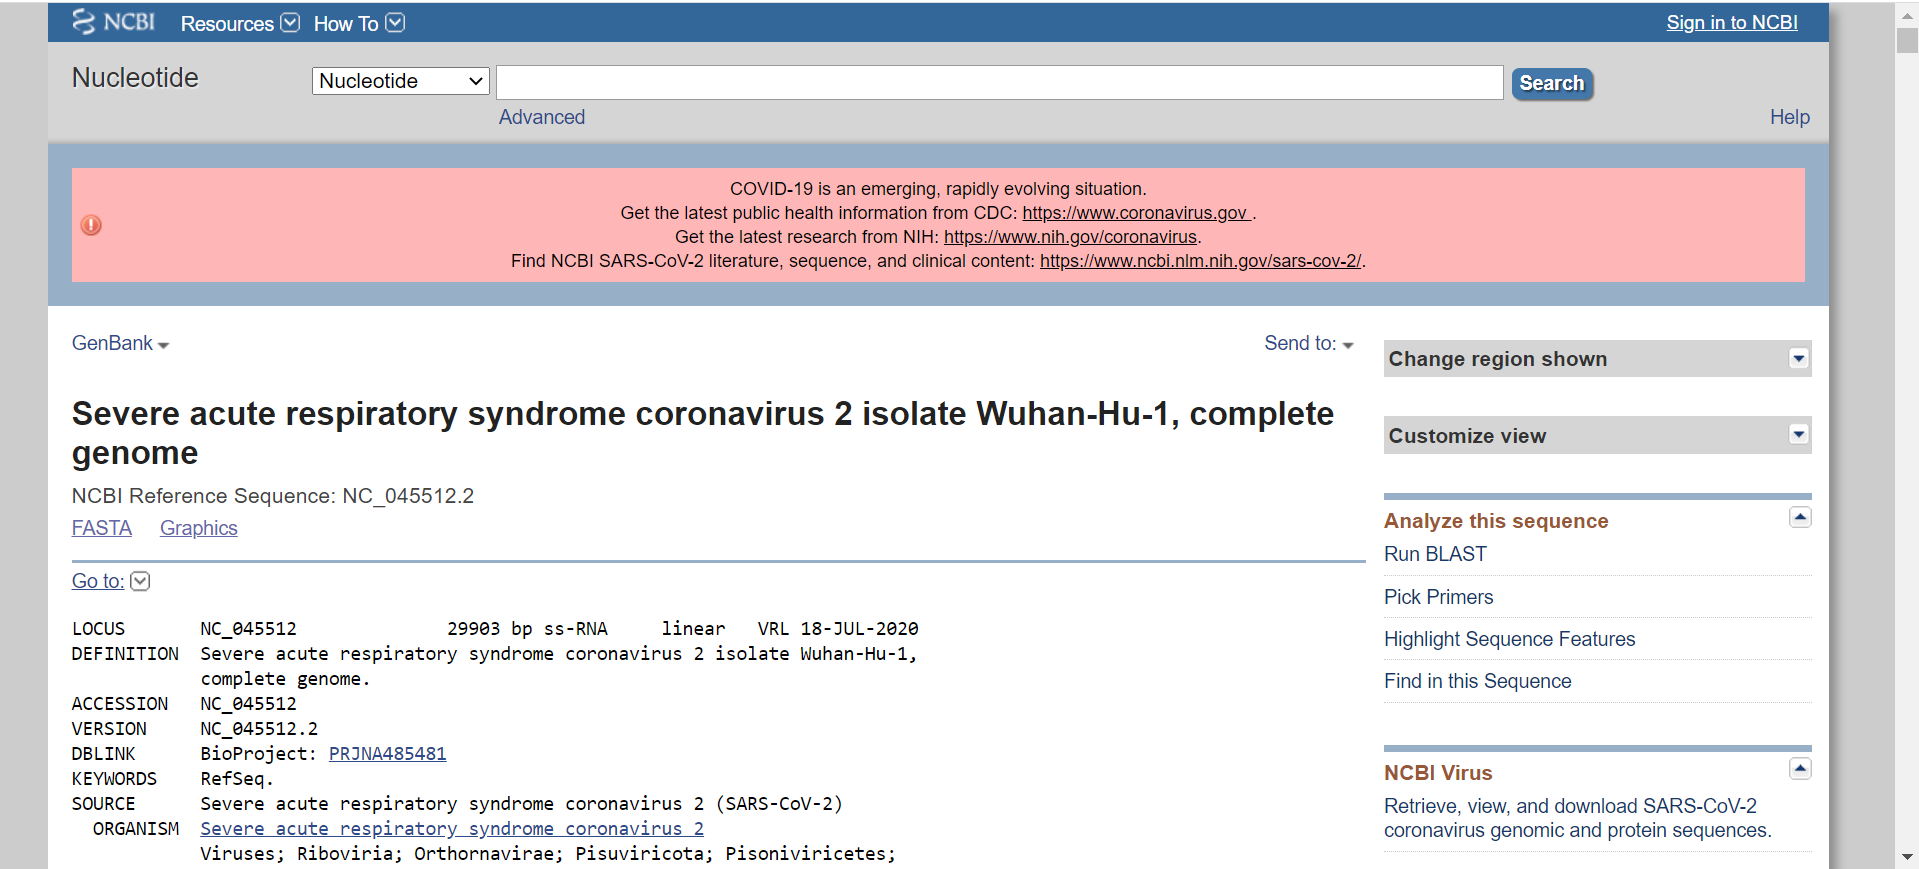
\includegraphics{./Images/img2.png}

In order to analyze the SARS-CoV-2 genome sequence in R, we need to
download the sequence in a \textbf{FASTA} format. The FASTA format is a
simple format for storing biological (DNA, RNA, and protein) sequences.
It begins with a single-line description starting with a
``\textgreater{}'' character followed by lines of sequences. Here is an
example of a FASTA file for a protein sequence:

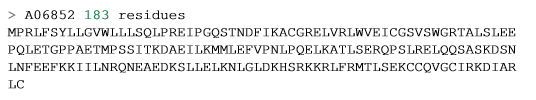
\includegraphics{./Images/img3.png}

To access the RNA sequence for SARS-CoV-2 from the Nucleotide database
as a FASTA format sequence file, click on the ``Send'' at the top right
of the NC\_045512.2 sequence record webpage, choose ``File'' in the
pop-up menu that appears, and then choose FASTA from the ``Format''
menu. Click ``Create file''. Name it sarscov2.fasta.

\#\#Interface with NCBI in R One can also carry out searches directly
from R using the SeqinR package. The SeqinR package was written by the
same group that crated the ACNUC database in Lyon, France. The ACNUC
database brings together data from various sources from NCBI, UniProt,
and Ensembl, and makes them all very easy to search. For a complete list
of all the databases included in the SeqinR package, we can use the
\texttt{choosebank()} command:

\begin{Shaded}
\begin{Highlighting}[]
\FunctionTok{require}\NormalTok{(}\StringTok{"seqinr"}\NormalTok{) }\CommentTok{\#load SeqinR library}
\FunctionTok{choosebank}\NormalTok{()}
\end{Highlighting}
\end{Shaded}

We just saw all of the databases that we can search with SeqinR. Here
are three of the most important ones:

\begin{itemize}
\tightlist
\item
  ``genebank'' contains DNA and RNA sequences from the NCBI Sequence
  Database, except for certain classes of sequences such as draft genome
  sequence data from genome sequencing projects.\\
\item
  ``refseq'' contains DNA and RNA sequences from the curated part of the
  NCBI Sequence Database.\\
\item
  ``refseqViruses'' contains DNA, RNA, and protein sequences from
  viruses from RefSeq.
\end{itemize}

If there is a particular database we want to search, we simply name that
database in the \texttt{choosebank()} function. For example, if we
wanted to query the Genbank database, we would say:

\begin{Shaded}
\begin{Highlighting}[]
\FunctionTok{choosebank}\NormalTok{(}\StringTok{"genbank"}\NormalTok{)}
\end{Highlighting}
\end{Shaded}

After we are finished with all of the analysis for a sequence, if we
want to switch to another database to search, first we need to close our
current database:

\begin{Shaded}
\begin{Highlighting}[]
\FunctionTok{closebank}\NormalTok{()}
\end{Highlighting}
\end{Shaded}

Once we specify which database to search through, we have to tell R what
to look for. Luckily, the query() function is flexible, and we can
specify a variety of different parameters in our search. For example, if
we don't know the accession number, we can provide the name of the
organism we're interested in instead. Here is a list of some of the
arguments we can supply query():

\begin{longtable}[]{@{}
  >{\raggedright\arraybackslash}p{(\columnwidth - 4\tabcolsep) * \real{0.1786}}
  >{\raggedright\arraybackslash}p{(\columnwidth - 4\tabcolsep) * \real{0.1607}}
  >{\raggedright\arraybackslash}p{(\columnwidth - 4\tabcolsep) * \real{0.6607}}@{}}
\toprule()
\begin{minipage}[b]{\linewidth}\raggedright
Argument
\end{minipage} & \begin{minipage}[b]{\linewidth}\raggedright
Example
\end{minipage} & \begin{minipage}[b]{\linewidth}\raggedright
Restricts your search to sequences:
\end{minipage} \\
\midrule()
\endhead
``AC='' & ``AC=NC\_001477'' & To the given accession number \\
``SP='' & ``SP=Chlamydia'' & To the specified organism \\
``M='' & ``M=mRNA'' & To a specific type (eg mRNA) \\
``J='' & ``J=Nature'' & Described in a specific journal \\
``R='' & ``R=Nature/460/352'' & Described in a paper in a particular
journal, volume, and start page \\
``AU='' & ``AU=Smith'' & Described in a paper or submitted to NCBI by a
specified author \\
\bottomrule()
\end{longtable}

We can combine these arguments with logical operators. Say we wanted to
find sequences published in the Nature journal by the author Smith. We
would combine the arguments like: ``J=Nature AND AU=Smith''. Other
important operators include OR and NOT. For more information, consult
the documentation page for the \texttt{query()} function. Say we wanted
to find the rabies genome sequence but we didn't know the accession
number. Since it's a virus, we would want to search ``refseqViruses''
database, so we would type the commands:

\begin{Shaded}
\begin{Highlighting}[]
\FunctionTok{choosebank}\NormalTok{(}\StringTok{"refseqViruses"}\NormalTok{)}
\NormalTok{rabies }\OtherTok{\textless{}{-}} \FunctionTok{query}\NormalTok{(}\StringTok{"SP=Rabies Virus"}\NormalTok{)}
\end{Highlighting}
\end{Shaded}

The results of our search are stored under the list variable rabies. The
query function gives us a list with six elements. To see what these
objects are named, type:

\begin{Shaded}
\begin{Highlighting}[]
\FunctionTok{attributes}\NormalTok{(rabies)}
\end{Highlighting}
\end{Shaded}

The content of each of these names is explained in the documentation
page of the \texttt{query()} function. For example, ``nelem'' contains
the number of sequences that match the query and ``req'' contains their
accession numbers.

\begin{Shaded}
\begin{Highlighting}[]
\NormalTok{rabies}\SpecialCharTok{$}\NormalTok{nelem[[}\DecValTok{1}\NormalTok{]]}
\end{Highlighting}
\end{Shaded}

\begin{Shaded}
\begin{Highlighting}[]
\NormalTok{rabies}\SpecialCharTok{$}\NormalTok{req[[}\DecValTok{1}\NormalTok{]]}
\end{Highlighting}
\end{Shaded}

The final step to retrieve a genomic sequence is to use the
\texttt{getSequence()} function to tell R to retrieve the sequence data.
Unlike the \texttt{query()} command, we need to know the accession
number. To get the sequence of rabies:

\begin{Shaded}
\begin{Highlighting}[]
\NormalTok{rabies\_seq }\OtherTok{\textless{}{-}} \FunctionTok{getSequence}\NormalTok{(rabies}\SpecialCharTok{$}\NormalTok{req[[}\DecValTok{1}\NormalTok{]])}
\FunctionTok{closebank}\NormalTok{() }\CommentTok{\#closes session}
\end{Highlighting}
\end{Shaded}

1.1 (a) Search the Genbank database for all human (\emph{Homo sapiens})
tRNA gene sequences. How many sequences match this query? \span

\begin{Shaded}
\begin{Highlighting}[]
\FunctionTok{require}\NormalTok{(}\StringTok{"seqinr"}\NormalTok{) }\CommentTok{\#load SeqinR library}
\end{Highlighting}
\end{Shaded}

\begin{verbatim}
## Loading required package: seqinr
\end{verbatim}

\begin{Shaded}
\begin{Highlighting}[]
\FunctionTok{choosebank}\NormalTok{(}\StringTok{"refseq"}\NormalTok{)}
\NormalTok{human }\OtherTok{\textless{}{-}} \FunctionTok{query}\NormalTok{(}\StringTok{"SP=Homo sapiens"}\NormalTok{)}
\NormalTok{human}\SpecialCharTok{$}\NormalTok{nelem[[}\DecValTok{1}\NormalTok{]]}
\end{Highlighting}
\end{Shaded}

\begin{verbatim}
## [1] 179103
\end{verbatim}

{ 179103 sequences match this query. }

(b) Pick any of these matches and save the gene sequence as the variable
tRNA\_seq. Find the length and GC content of the sequence. \span

\begin{Shaded}
\begin{Highlighting}[]
\NormalTok{accNum }\OtherTok{\textless{}{-}}\NormalTok{ human}\SpecialCharTok{$}\NormalTok{req[[}\DecValTok{1}\NormalTok{]]}
\NormalTok{tRNA\_seq }\OtherTok{\textless{}{-}} \FunctionTok{getSequence}\NormalTok{(human}\SpecialCharTok{$}\NormalTok{req[[}\DecValTok{1}\NormalTok{]])}

\FunctionTok{length}\NormalTok{(tRNA\_seq)}
\end{Highlighting}
\end{Shaded}

\begin{verbatim}
## [1] 4945
\end{verbatim}

\begin{Shaded}
\begin{Highlighting}[]
\FunctionTok{GC}\NormalTok{(tRNA\_seq)}
\end{Highlighting}
\end{Shaded}

\begin{verbatim}
## [1] 0.4859454
\end{verbatim}

\begin{Shaded}
\begin{Highlighting}[]
\FunctionTok{closebank}\NormalTok{()}
\end{Highlighting}
\end{Shaded}

{ The length and GC content of the sequence is 4945 and 0.486
respectively. }

(c) What is the function of tRNA? (a Google search can help) \span

{ tRNA serves as a link between the mRNA molecule and the growing chain
of amino acids that make up a protein }

1.2 It is important that you know how to find biological data, such as
sequences. Doing that, as you saw in assignment, involves accessing a
database. But there are many databases with different information, and
different databases might handle their entries differently, or be more
specialized. What is the difference between NCBI's
\href{https://www.ncbi.nlm.nih.gov/genbank/}{Genbank} and
\href{https://www.ncbi.nlm.nih.gov/refseq/}{RefSeq}? \span 

{ RefSeq is limited to major organisms for which sufficient data are
available. GenBank includes sequences for any organism submitted. }

Now that you know how to use R to pull genetic data, let's practice
making functions to analyze genetic sequences.

\hypertarget{part-2-open-reading-frames-orfs}{%
\subsection{Part 2: Open Reading Frames
(ORFs)}\label{part-2-open-reading-frames-orfs}}

\hypertarget{the-central-dogma-of-molecular-biology}{%
\paragraph{The Central Dogma of molecular
biology}\label{the-central-dogma-of-molecular-biology}}

Our genes contain the blueprint for our cells and our bodies. In today's
world, this is common knowledge. But what may be less obvious is exactly
\emph{how} those sequences of DNA exert their effects in the physical,
biological world. The short story is that the plan contained in DNA is
put into action by proteins, but this idea brings us to a fundamental
teaching in modern biology: \textbf{the central dogma of molecular
biology}. As originally stated in Francis Crick's (of Watson and Crick
fame) 1958
\href{https://profiles.nlm.nih.gov/spotlight/sc/feature/doublehelix}{paper}
``On Protein Synthesis'', the central dogma \emph{``\ldots states that
once `information' has passed into protein it cannot get out again. In
more detail, the transfer of information from nucleic acid to nucleic
acid, or from nucleic acid to protein may be possible, but transfer from
protein to protein, or from protein to nucleic acid is impossible.
Information means here the precise determination of sequence, either of
bases in the nucleic acid or of amino acid residues in the protein.''}

A consequence of this statement--with the benefit of some additional
information from experimental biology since 1958--is the following:
\textbf{The flow of information during protein synthesis is \emph{from
DNA to RNA to Protein}}. We've touched upon DNA and proteins, but what
is this RNA intermediary? The first step on the path from DNA to protein
is for the double-stranded DNA to be \textbf{transcribed} to form a
single-stranded mRNA (messenger RNA) molecule. A big benefit of this
transcription step is that \emph{many mRNA molecules can be repeatedly
transcribed from DNA}, allowing for \textbf{amplification}.

To illustrate the benefits of amplification, imagine if every high
schooler in the United States had to be taught biology from a
\emph{single physical copy} of a textbook. Learning anything would be
practically impossible! Similarly, if proteins were created directly
from DNA, then the resulting traffic jam in the nuclei of our cells
would make cellular processes slow to a crawl. Instead, by first
transcribing to an mRNA intermediary, cells are able to quickly
manufacture key proteins in large quantities. We are able to make
photocopies of that precious, precious textbook.

However, we encounter a slight problem, because there are four nucleic
acids used in our genetic code (ATCG for DNA, AUCG for RNA), but there
are 20 (sometimes more!) amino acids used in the construction of our
proteins. A one-to-one translation would be clearly impossible. Instead,
to translate from mRNA to protein, \textbf{three nucleotides code for
one amino acid}. Strings of these \textbf{triplet codons} form the
\textbf{protein-coding regions} of our genes. A table of codons follows:

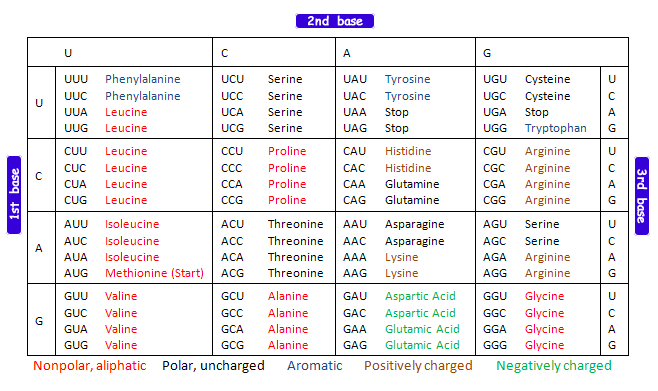
\includegraphics{./Images/codontable.png}

So there is the mRNA code to protein code translation problem solved.
But how do we know where the protein-coding regions begin? Another
problem. There are many different markers that tell us where
protein-coding regions reside in our genomes, but a basic and important
one that helps us to predict the locations is the concept of the
\textbf{open reading frame} or \textbf{ORF}, a string of nucleotides
that starts with a \textbf{start (AUG)} codon and ends with a
\textbf{stop (TAA, or TAG, or TGA)} codon. We will be implementing an
algorithm to find all ORFs with some minimum length in a given
nucleotide sequence below. In support of this endeavor, we will write a
few helper functions now.

2.1 a) Write a function that takes in a gene sequence and stores the
indices of the first nucleotide of the start codon in the vector
\texttt{startcodons}, and returns this vector at the end. Note that the
DNA sequences we will use will contain lower case characters,
i.e.~``a'', ``t'', ``g'', ``c''. The last 2 lines in the chunk will test
your \texttt{findStartCodons()} function on a sample sequence called
\texttt{seq}. Pseudocode is given below to help guide you, but you are
free to write in your own style. \emph{Hint: use a nested if statement
inside a for loop to iterate over the entire sequence and evaluate
whether the letters are ``a'', ``t'', ``g'' using truth statements
(\texttt{\&\&} and \texttt{==}). USE LOWERCASE LETTERS} \span

\begin{Shaded}
\begin{Highlighting}[]
\NormalTok{findStartCodons }\OtherTok{\textless{}{-}} \ControlFlowTok{function}\NormalTok{(seq)\{}
\NormalTok{  startcodons }\OtherTok{\textless{}{-}} \FunctionTok{numeric}\NormalTok{(}\DecValTok{0}\NormalTok{) }\CommentTok{\#This will initiate an empty vector. You can index into this vector at any location to store a new value. I.e. to store a value of 100 in the first position of this vector, you would index into the first location in \textasciigrave{}startcodons\textasciigrave{} and set it equal to 100.}
\NormalTok{  k }\OtherTok{\textless{}{-}} \DecValTok{1} \CommentTok{\#use k to index the \textquotesingle{}startcodons\textquotesingle{} vector (startcodons[k]) as you store in it the index of each start codon you find in \textquotesingle{}seq\textquotesingle{}. Remember to increase k each time (k\textless{}{-}k+1). }
  \ControlFlowTok{for}\NormalTok{(i }\ControlFlowTok{in} \DecValTok{1}\SpecialCharTok{:}\NormalTok{(}\FunctionTok{length}\NormalTok{(seq)}\SpecialCharTok{{-}}\DecValTok{5}\NormalTok{))\{}
    \ControlFlowTok{if}\NormalTok{(seq[i] }\SpecialCharTok{==} \StringTok{"a"} \SpecialCharTok{\&\&}\NormalTok{ seq[i}\SpecialCharTok{+}\DecValTok{1}\NormalTok{] }\SpecialCharTok{==} \StringTok{"t"} \SpecialCharTok{\&\&}\NormalTok{ seq[i}\SpecialCharTok{+}\DecValTok{2}\NormalTok{] }\SpecialCharTok{==} \StringTok{"g"}\NormalTok{) \{}
\NormalTok{      startcodons[k] }\OtherTok{\textless{}{-}}\NormalTok{ i}
\NormalTok{      k }\OtherTok{\textless{}{-}}\NormalTok{ k }\SpecialCharTok{+} \DecValTok{1}
\NormalTok{    \}}
\NormalTok{  \}}
  \FunctionTok{return}\NormalTok{(startcodons)}
\NormalTok{\}}

\CommentTok{\#Testing the function}
\NormalTok{seq}\OtherTok{\textless{}{-}}\FunctionTok{c}\NormalTok{(}\StringTok{"g"}\NormalTok{, }\StringTok{"t"}\NormalTok{, }\StringTok{"a"}\NormalTok{, }\StringTok{"a"}\NormalTok{, }\StringTok{"t"}\NormalTok{, }\StringTok{"g"}\NormalTok{, }\StringTok{"t"}\NormalTok{, }\StringTok{"a"}\NormalTok{, }\StringTok{"g"}\NormalTok{, }\StringTok{"t"}\NormalTok{, }\StringTok{"g"}\NormalTok{, }\StringTok{"a"}\NormalTok{, }\StringTok{"t"}\NormalTok{, }\StringTok{"t"}\NormalTok{, }\StringTok{"g"}\NormalTok{, }\StringTok{"t"}\NormalTok{, }\StringTok{"a"}\NormalTok{, }\StringTok{"g"}\NormalTok{)}
\FunctionTok{findStartCodons}\NormalTok{(seq)}
\end{Highlighting}
\end{Shaded}

\begin{verbatim}
## [1] 4
\end{verbatim}

In 2.1(b), The for loop iterated over \texttt{1:(length(seq)-5)},whereas
in 2.1(c), it will iterate over \texttt{1:(length(seq)-2)}.. Explain the
logic behind this difference. (Hint: to understand
\texttt{1:(length(seq)-5)} in 1c, think about where the start and stop
codons must fall in order for them to create an open reading frame.)
\span

{ There cannot be a start codon as the last codon in the DNA sequence.
So we don't need to search the last codon, as there is no chance for it
to be a start. However, the last codon may be a stop codon. }

2.1 c) Write a function that takes in a gene sequence and stores the
indices of the first nucleotide of stop codons in the vector
\texttt{stopcodons}, and return this vector at the end. Pseudocode is
given below to help guide you, but you are free to write in your own
style. Remember that there are three different stop codons! \emph{Hint:
some ways of doing this include using the OR statement
(\texttt{\textbar{}\textbar{}}), or multiple if statements.}\span

\begin{Shaded}
\begin{Highlighting}[]
\CommentTok{\# This function receives a DNA sequence as input and outputs a vector with the position of all stop codons.}

\NormalTok{findStopCodons }\OtherTok{\textless{}{-}} \ControlFlowTok{function}\NormalTok{(seq)\{}
\NormalTok{  stopcodons }\OtherTok{\textless{}{-}}\FunctionTok{numeric}\NormalTok{(}\DecValTok{0}\NormalTok{)}\CommentTok{\#This will initiate an empty vector. You can index into this vector at any location to store a new value. For example, to store a value of 100 in the first position of this vector, you would index into the first location in stopcodons and set it equal to 100.}
\NormalTok{  k }\OtherTok{\textless{}{-}} \DecValTok{1}
  \ControlFlowTok{for}\NormalTok{(i }\ControlFlowTok{in} \DecValTok{1}\SpecialCharTok{:}\NormalTok{(}\FunctionTok{length}\NormalTok{(seq)}\SpecialCharTok{{-}}\DecValTok{2}\NormalTok{))\{ }
    \CommentTok{\# check for TAA}
    \ControlFlowTok{if}\NormalTok{(seq[i] }\SpecialCharTok{==} \StringTok{"t"} \SpecialCharTok{\&\&}\NormalTok{ seq[i}\SpecialCharTok{+}\DecValTok{1}\NormalTok{] }\SpecialCharTok{==} \StringTok{"a"} \SpecialCharTok{\&\&}\NormalTok{ seq[i}\SpecialCharTok{+}\DecValTok{2}\NormalTok{] }\SpecialCharTok{==} \StringTok{"a"}\NormalTok{) \{}
\NormalTok{      stopcodons[k] }\OtherTok{\textless{}{-}}\NormalTok{ i}
\NormalTok{      k }\OtherTok{\textless{}{-}}\NormalTok{ k }\SpecialCharTok{+} \DecValTok{1}
\NormalTok{    \}}
    
    \CommentTok{\# check for TAG}
    \ControlFlowTok{if}\NormalTok{(seq[i] }\SpecialCharTok{==} \StringTok{"t"} \SpecialCharTok{\&\&}\NormalTok{ seq[i}\SpecialCharTok{+}\DecValTok{1}\NormalTok{] }\SpecialCharTok{==} \StringTok{"a"} \SpecialCharTok{\&\&}\NormalTok{ seq[i}\SpecialCharTok{+}\DecValTok{2}\NormalTok{] }\SpecialCharTok{==} \StringTok{"g"}\NormalTok{) \{}
\NormalTok{      stopcodons[k] }\OtherTok{\textless{}{-}}\NormalTok{ i}
\NormalTok{      k }\OtherTok{\textless{}{-}}\NormalTok{ k }\SpecialCharTok{+} \DecValTok{1}
\NormalTok{    \}}
    
    \CommentTok{\# check for TGA}
    \ControlFlowTok{if}\NormalTok{(seq[i] }\SpecialCharTok{==} \StringTok{"t"} \SpecialCharTok{\&\&}\NormalTok{ seq[i}\SpecialCharTok{+}\DecValTok{1}\NormalTok{] }\SpecialCharTok{==} \StringTok{"g"} \SpecialCharTok{\&\&}\NormalTok{ seq[i}\SpecialCharTok{+}\DecValTok{2}\NormalTok{] }\SpecialCharTok{==} \StringTok{"a"}\NormalTok{) \{}
\NormalTok{      stopcodons[k] }\OtherTok{\textless{}{-}}\NormalTok{ i}
\NormalTok{      k }\OtherTok{\textless{}{-}}\NormalTok{ k }\SpecialCharTok{+} \DecValTok{1}
\NormalTok{    \}}
\NormalTok{  \}}
  \FunctionTok{return}\NormalTok{(stopcodons)}
\NormalTok{\}}
\CommentTok{\#Testing the function}
\NormalTok{seq}\OtherTok{\textless{}{-}}\FunctionTok{c}\NormalTok{(}\StringTok{"g"}\NormalTok{, }\StringTok{"t"}\NormalTok{, }\StringTok{"a"}\NormalTok{, }\StringTok{"a"}\NormalTok{, }\StringTok{"t"}\NormalTok{, }\StringTok{"g"}\NormalTok{, }\StringTok{"t"}\NormalTok{, }\StringTok{"a"}\NormalTok{, }\StringTok{"g"}\NormalTok{, }\StringTok{"t"}\NormalTok{, }\StringTok{"g"}\NormalTok{, }\StringTok{"a"}\NormalTok{, }\StringTok{"t"}\NormalTok{, }\StringTok{"t"}\NormalTok{, }\StringTok{"g"}\NormalTok{, }\StringTok{"t"}\NormalTok{, }\StringTok{"a"}\NormalTok{, }\StringTok{"g"}\NormalTok{)}
\FunctionTok{findStopCodons}\NormalTok{(seq)}
\end{Highlighting}
\end{Shaded}

\begin{verbatim}
## [1]  2  7 10 16
\end{verbatim}

A large number of protein sequences start with Methionine. From the the
table above, we can see that the codon for Methionine is AUG (ATG in DNA
code), and is also labeled as ``Start''. But Methionine is also an
important amino acid \emph{within} protein structures. How do we then
determine where a protein begins? The truth is that, based on the
genetic code alone, this is a difficult task. But we can predict where
protein-coding regions begin and end because all protein sequences also
end in one of three codons: UAA, UAG, or UGA (TAA, TAG, and TGA in DNA
code). These are the \textbf{stop codons}. They do not normally code for
amino acids but rather serve to signify that translation of the protein
will terminate at that position. \textbf{\emph{If a stop codon is
encountered by protein-forming machinery, then translation }will stop}.

So a structure for an open reading frame begins to appear: a start
codon, some number of intervening codons that code for the amino acids
of the protein, and a stop codon to terminate the sequence. All of these
components are formed from three-nucleotide codons, so a key property of
these frames is that \textbf{their length in nucleotides is evenly
divisible by 3}.\span

\textbf{But there is another problem. There are three different
``frames'' possible for a given direction. To explain:} Consider the
sequence ``GTCATGAT''. If we start from the first nucleotide ``G'' and
start assigning codons, then we get the following: \textbf{(frame 1) GTC
ATG, or Valine Methionine}. Let's start at the second nucleotide:
\textbf{(frame 2) TCA TGA, or Serine STOP}. And if we start at
nucleotide 3: \textbf{(frame 3) CAT GAT, or Histidine Aspartate}. Note
that if we start at the fourth nucleotide, we are \textbf{\emph{in
reading frame 1 once again}}: ATG. All of this also applies to the
complementary strand, so for a double-stranded genome, there are six
possible reading frames.

From this, we can see that if we want our open readng frames to begin
with our start codon (ATG) and end with one of our stop codons (TAA,
TAG, or TGA), then we will need our start and stop codons to be
\textbf{in the same reading frame}. Put simply, this means that the
length spanned by our open reading frame (first nucleotide of start
codon to final nucleotide of our stop codon) must be evenly divisible by
3.

Now we're getting somewhere. Another condition is the ability to store
the longest ORFs for each unique stop codon in the case where multiple
start codons could theoretically pair with that stop codon to form valid
ORFs. A final condition is that our ORFs \textbf{must be of some minimum
length with no intervening in-frame stop codons.} This means that our
ORFs must code for a certain number of amino acids so that the product
will be a polypeptide of significant length. If there is a stop codon
in-frame between our chosen start and stop codons, then that ORF would
terminate by definition at that intervening stop codon, so our putative
ORF is not valid.

To summarize, our general strategy is delineated below:

\begin{enumerate}
\def\labelenumi{\arabic{enumi})}
\tightlist
\item
  Determine the index for all the start codons for a given reading frame
\item
  Determine the index for all the stop codons for a given reading frame
\item
  For each start codon, find the nearest stop codon (that comes after
  the start codon). If the stop codon fulfills all requirements
  (in-frame, over the minimum length), store as ORF.
\item
  Start at the next start codon AFTER the last stop codon.
\item
  Repeat for all reading frames
\end{enumerate}

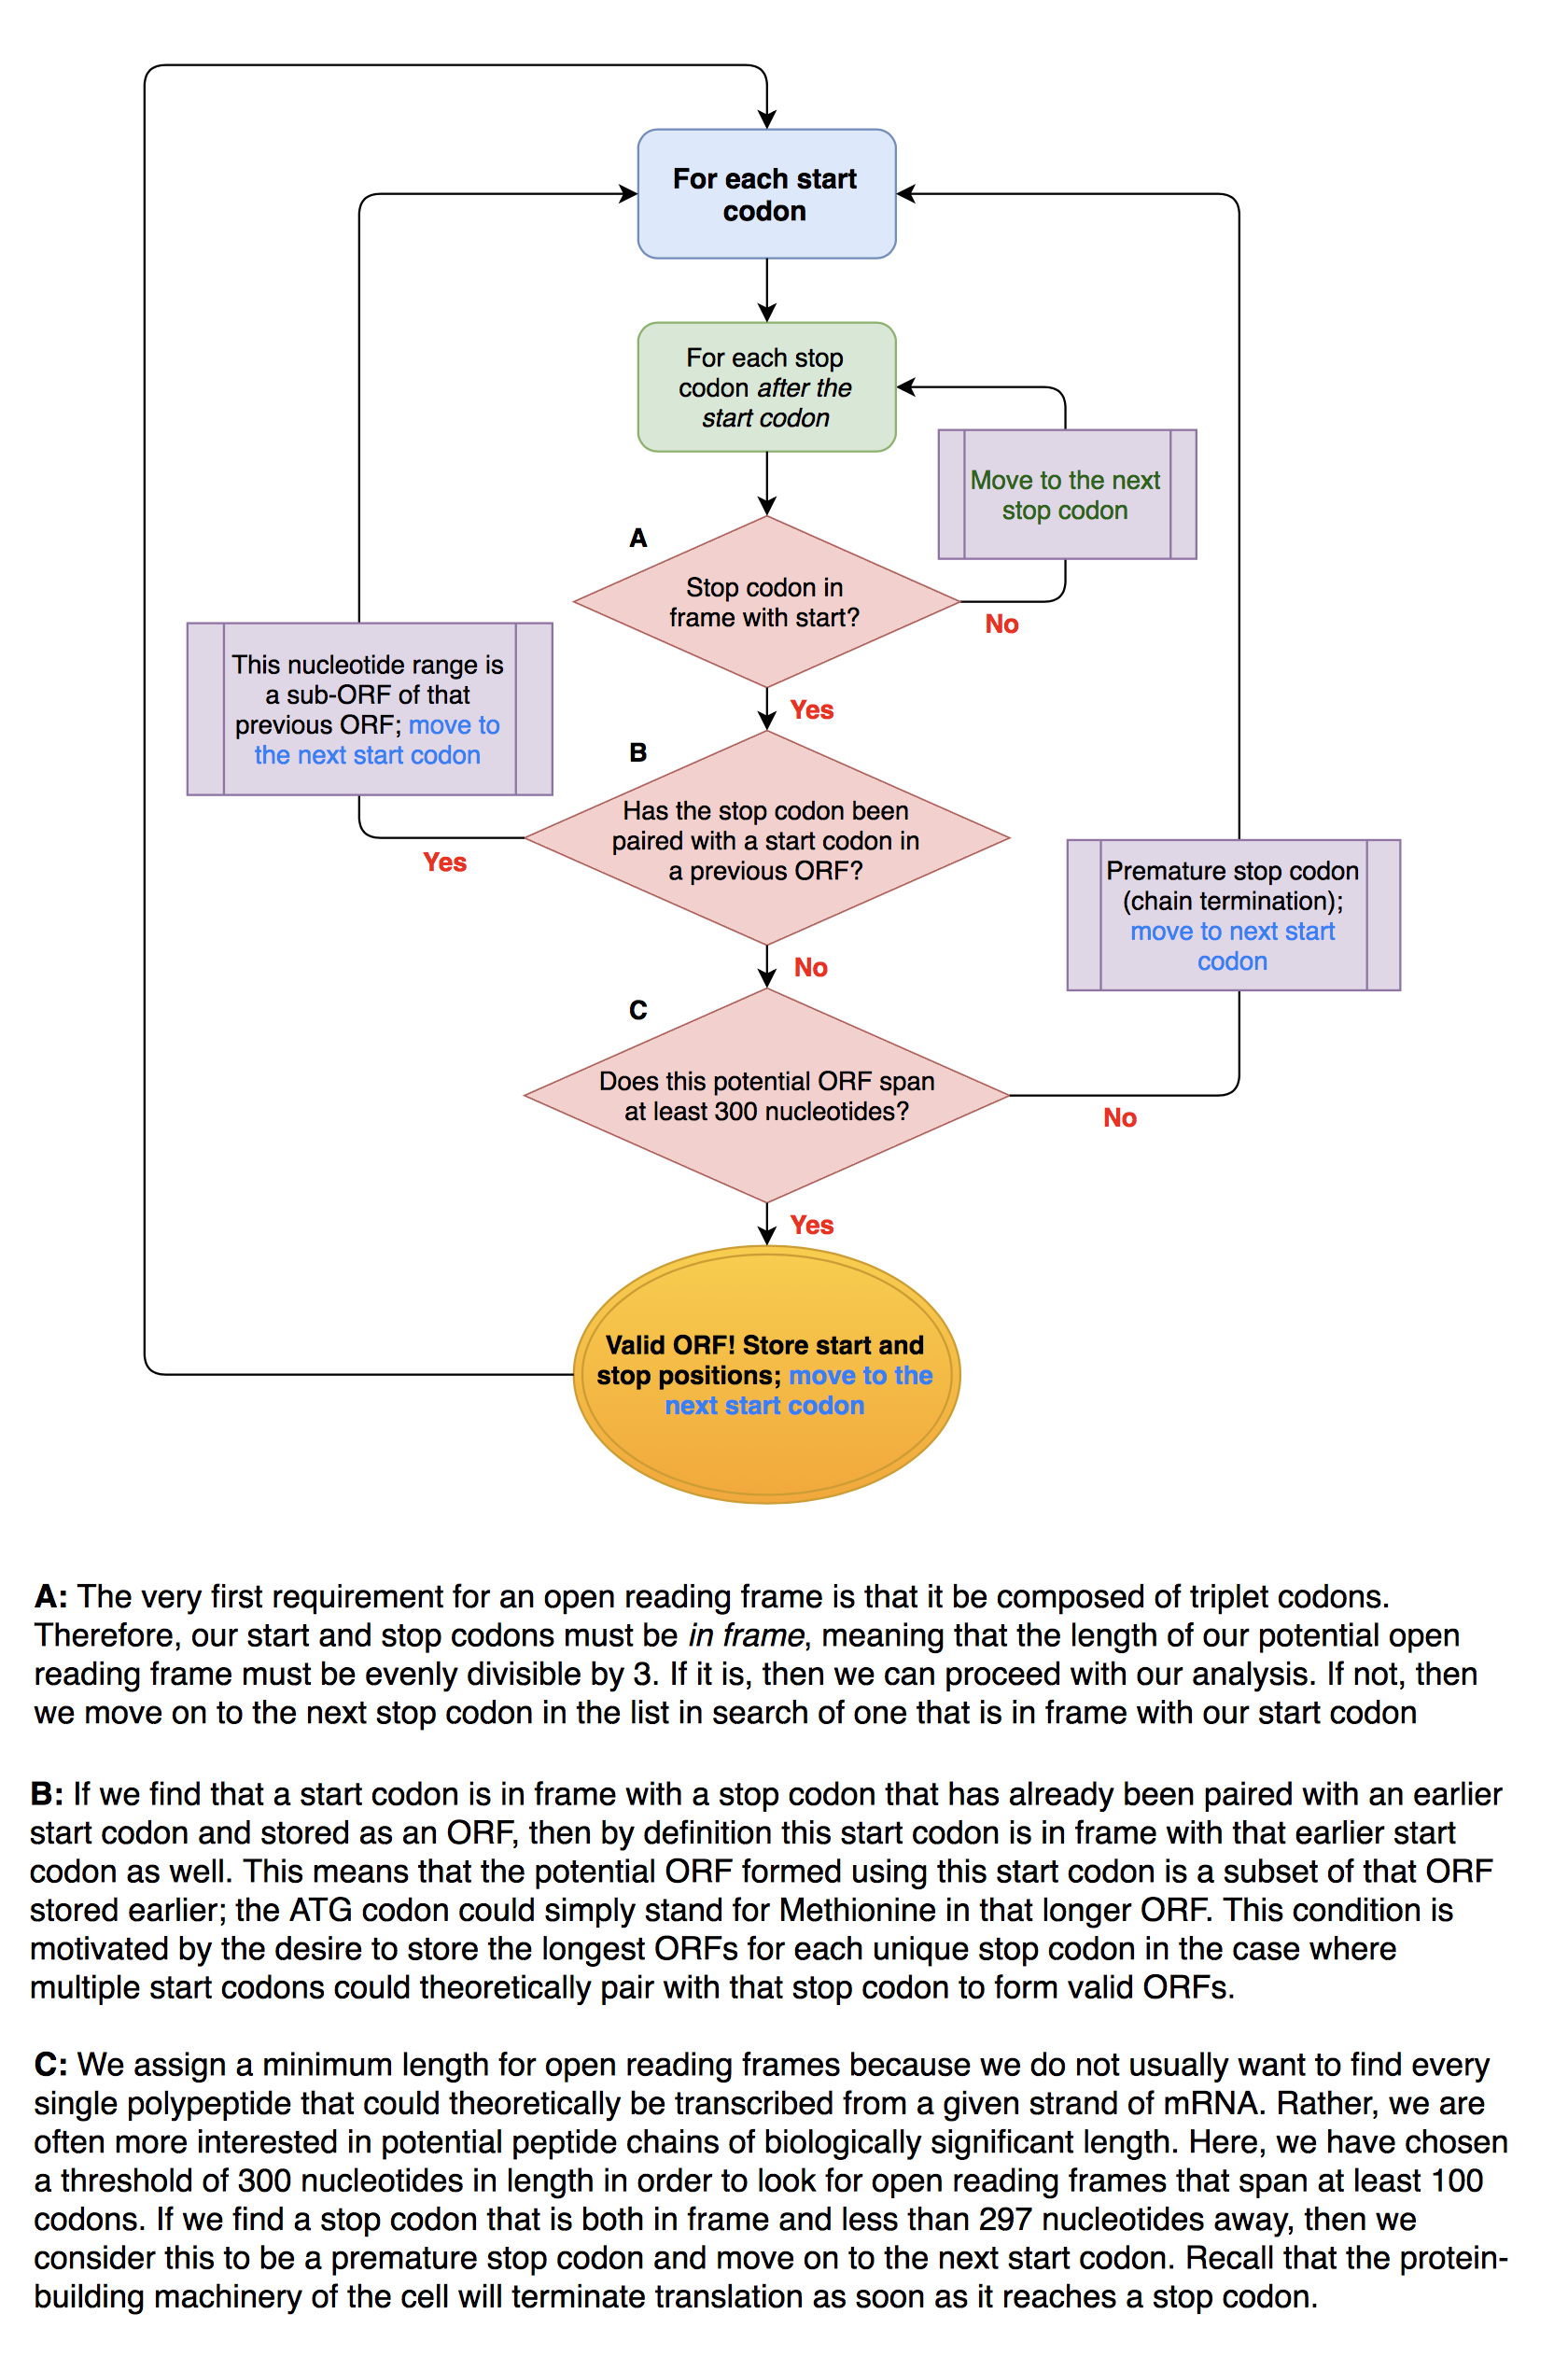
\includegraphics{./Images/ORF.png}

2.2 Write a function to find possible open reading frames (ORFs) in a
given sequence. Let us define those to be a substring starting with the
start codon ``AUG'' and ending with one of the stop codons and whose
length is divisible by 3 so it can be a coding sequence without any
intervening in-frame stop codons. Also, store the longest ORFs for each
unique stop codon in the case where multiple start codons could
theoretically pair with that stop codon to form valid ORFs. The inputs
should be a nucleotide sequence and a minimum length in codons, and the
output should be a character vector containing strings of the following
format (see \texttt{?paste}):
\texttt{"\textless{}first\ base\ of\ start\textgreater{}\ to\ \textless{}last\ base\ of\ stop\textgreater{}"}
(i.e.~\texttt{"409\ to\ 1273"}). A pseudocode sketch of a possible code
implementation is below: \span

\begin{Shaded}
\begin{Highlighting}[]
\NormalTok{findORF }\OtherTok{\textless{}{-}} \ControlFlowTok{function}\NormalTok{(sequence, minLength) \{}
\NormalTok{    ORFs }\OtherTok{\textless{}{-}} \FunctionTok{character}\NormalTok{()}
\NormalTok{    startInds }\OtherTok{\textless{}{-}} \FunctionTok{findStartCodons}\NormalTok{(sequence)}
\NormalTok{    stopInds }\OtherTok{\textless{}{-}} \FunctionTok{findStopCodons}\NormalTok{(sequence)}
    \CommentTok{\# loop through each reading frame}
    \ControlFlowTok{for}\NormalTok{(i }\ControlFlowTok{in} \DecValTok{1}\SpecialCharTok{:}\DecValTok{3}\NormalTok{) \{}
\NormalTok{        indexStart }\OtherTok{\textless{}{-}}\NormalTok{ i}
        \ControlFlowTok{while}\NormalTok{ (indexStart }\SpecialCharTok{\textless{}}\NormalTok{ (}\FunctionTok{length}\NormalTok{(sequence)}\SpecialCharTok{{-}}\NormalTok{minLength}\SpecialCharTok{*}\DecValTok{3}\SpecialCharTok{+}\DecValTok{1}\NormalTok{)) \{}
            \ControlFlowTok{if}\NormalTok{(indexStart }\SpecialCharTok{\%in\%}\NormalTok{ startInds) \{}
\NormalTok{                numCodons }\OtherTok{\textless{}{-}} \DecValTok{2} \CommentTok{\#for the start codon and the first codon considered in the following iteration}
\NormalTok{                firstPossStop }\OtherTok{\textless{}{-}}\NormalTok{ indexStart }\SpecialCharTok{+} \DecValTok{3}\SpecialCharTok{*}\NormalTok{numCodons}
                \ControlFlowTok{for}\NormalTok{(indexStop }\ControlFlowTok{in} \FunctionTok{seq}\NormalTok{(firstPossStop,}\FunctionTok{length}\NormalTok{(sequence),}\AttributeTok{by=}\DecValTok{3}\NormalTok{)) \{}
                    \ControlFlowTok{if}\NormalTok{(indexStop }\SpecialCharTok{\%in\%}\NormalTok{ stopInds) \{}
                        \ControlFlowTok{if}\NormalTok{(numCodons }\SpecialCharTok{\textgreater{}=}\NormalTok{ minLength) \{}
\NormalTok{                            currORF }\OtherTok{\textless{}{-}} \FunctionTok{paste}\NormalTok{(indexStart, }\StringTok{"to"}\NormalTok{, indexStop}\SpecialCharTok{+}\DecValTok{2}\NormalTok{, }\AttributeTok{sep=}\StringTok{" "}\NormalTok{)}
\NormalTok{                            ORFs }\OtherTok{\textless{}{-}} \FunctionTok{append}\NormalTok{(ORFs, currORF)}
\NormalTok{                        \}}
\NormalTok{                        indexStart }\OtherTok{\textless{}{-}}\NormalTok{ indexStop}
                        \ControlFlowTok{break}
\NormalTok{                    \}}
\NormalTok{                    numCodons }\OtherTok{\textless{}{-}}\NormalTok{ numCodons }\SpecialCharTok{+} \DecValTok{1}
\NormalTok{                \}}
\NormalTok{            \}}
\NormalTok{            indexStart }\OtherTok{\textless{}{-}}\NormalTok{ indexStart }\SpecialCharTok{+} \DecValTok{3}
\NormalTok{        \}}
\NormalTok{    \}}
    \FunctionTok{return}\NormalTok{(ORFs)}
\NormalTok{\}}
\end{Highlighting}
\end{Shaded}

\texttt{break} statements are used inside a loop to basically break out
of it. It does not return a value; it stops the iterations and transfers
the control of the loop to outside of the loop. In a nested loop, the
statement exits from the inner-most loop to the first statement outside.

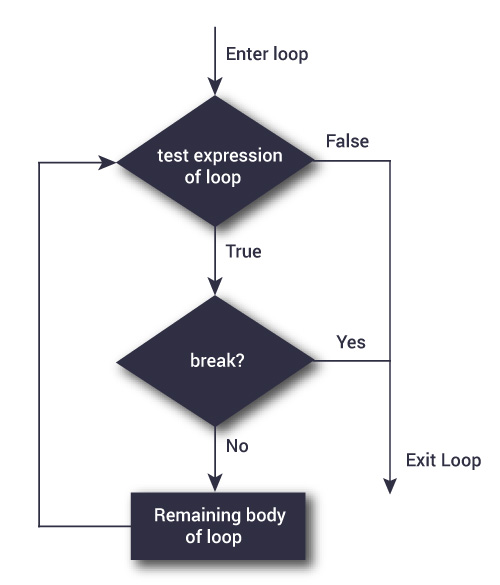
\includegraphics{./Images/img4.jpg}

2.3. Use the function you wrote above to calculate the possible ORFs
with a minimum length of 200 (triplet, 600 nucleotides) codons in the
Zika virus genome. Please \textbf{display your results}. Note: You will
need to \textbf{load the genome} (stored in `Zika.fasta') into R using
\texttt{read.fasta()} from \texttt{library(seqinr)}. \span

\begin{Shaded}
\begin{Highlighting}[]
\CommentTok{\# load the zika virus sequence}
\FunctionTok{library}\NormalTok{(}\StringTok{"seqinr"}\NormalTok{)}
\NormalTok{zika }\OtherTok{\textless{}{-}} \FunctionTok{read.fasta}\NormalTok{(}\AttributeTok{file =} \StringTok{"Sequences/zika.fasta"}\NormalTok{)}
\NormalTok{zika\_seq }\OtherTok{\textless{}{-}}\NormalTok{ zika[[}\DecValTok{1}\NormalTok{]]}

\FunctionTok{findORF}\NormalTok{(zika\_seq, }\DecValTok{200}\NormalTok{)}
\end{Highlighting}
\end{Shaded}

\begin{verbatim}
## [1] "107 to 10366"
\end{verbatim}

2.4. Do you find the number of ORFs surprising \textbf{considering the
number of proteins coded by the virus}? Do some research into how the
zika genome is organized and expressed (you may find
\href{http://viralzone.expasy.org/6756?outline=all_by_species}{this
page} useful). With this information in mind, justify the number of ORFs
you found in question 2.3. (Note: pay attention to the biological
mechanism of the genome expression.) \span

{ Yes, I find it surprising that there is only one ORF in the genome
considering the number of proteins coded for by the virus. The whole
genome is translated into one large protein, which is then processed co-
and post-translationally by host and viral proteases. }

2.5 Use the function you wrote above to calculate the possible ORFs
(minimum length of 100, that is, 300 nucleotides) in the coronavirus
genome. Note: You will need to \textbf{load the genome} (stored in
`covid19.fasta') into R using \texttt{read.fasta()} from
\texttt{library(seqinr)}. \span

\begin{Shaded}
\begin{Highlighting}[]
\CommentTok{\# load the covid19 virus sequence}
\FunctionTok{library}\NormalTok{(}\StringTok{"seqinr"}\NormalTok{)}
\NormalTok{covid19 }\OtherTok{\textless{}{-}} \FunctionTok{read.fasta}\NormalTok{(}\AttributeTok{file =} \StringTok{"Sequences/covid19.fasta"}\NormalTok{)}
\NormalTok{covid19\_seq }\OtherTok{\textless{}{-}}\NormalTok{ covid19[[}\DecValTok{1}\NormalTok{]]}

\FunctionTok{findORF}\NormalTok{(covid19\_seq, }\DecValTok{100}\NormalTok{)}
\end{Highlighting}
\end{Shaded}

\begin{verbatim}
## [1] "13768 to 21555" "25393 to 26220" "27394 to 27759" "266 to 13483"  
## [5] "21536 to 25384" "28274 to 29533" "26523 to 27191" "27894 to 28259"
\end{verbatim}

2.6 Do you find the number of ORFs surprising in in the coronavirus
genome \textbf{considering the number of proteins coded by the virus}?
Do some research into how the coronavirus genome is organized and
expressed (you may find
\href{https://www-ncbi-nlm-nih-gov.proxy.uchicago.edu/pmc/articles/PMC7525243/}{this
page} useful). With this information in mind, justify the number of ORFs
you found in question 2.5. \span

{ DO THIS LATER }

2.7 Use the function you wrote above to calculate the possible ORFs
(minimum length 50, that is, 150 nucleotides) in the HIV virus genome.
Note: You will need to load the genome (stored in `HIV.fasta') into R
using \texttt{read.fasta()} from \texttt{library(seqinr)}. Compare the
number of ORFs you find to the number of genes known to be encoded by
the HIV genome. Propose a reason for how there are more proteins
produced by HIV than the number of its genes.\span

\begin{Shaded}
\begin{Highlighting}[]
\CommentTok{\# load the HIV sequence}
\FunctionTok{library}\NormalTok{(}\StringTok{"seqinr"}\NormalTok{)}
\NormalTok{hiv }\OtherTok{\textless{}{-}} \FunctionTok{read.fasta}\NormalTok{(}\AttributeTok{file =} \StringTok{"Sequences/HIV.fasta"}\NormalTok{)}
\NormalTok{hiv\_seq }\OtherTok{\textless{}{-}}\NormalTok{ hiv[[}\DecValTok{1}\NormalTok{]]}

\FunctionTok{findORF}\NormalTok{(hiv\_seq, }\DecValTok{50}\NormalTok{)}
\end{Highlighting}
\end{Shaded}

\begin{verbatim}
##  [1] "3955 to 4122" "5377 to 5595" "5608 to 5856" "797 to 955"   "1904 to 4642"
##  [6] "5105 to 5341" "5771 to 8341" "336 to 1838"  "4587 to 5165" "8343 to 8714"
\end{verbatim}

{ One reason that there are more proteins produced by HIV than the
number of its genes is because of alternative RNA splicing. This is the
process of selecting different exons to actually be spliced together to
the final mRNA that gets translated into the protein. This can allow for
a single gene to code for multiple different proteins depending on the
combination of exons spliced together. }

\hypertarget{part-3-finding-oric}{%
\subsection{\texorpdfstring{Part 3: Finding
\emph{oriC}}{Part 3: Finding oriC}}\label{part-3-finding-oric}}

The next question tries to use the tools you have learned and developed
to try to address the question: Where is the origin of DNA replication?

Watch the DNA replication video in the lab folder. \span

We will try to do this in the bacterial genome, which usually has only
one chromosome. The bacterial genome, different from that of animals,
plants, fungi and archaea, is usually circular. This slightly
complicates its analysis, since there isn't a point where it starts or
ends, and it isn't easy to handle circular data. Hence, we are going to
handle bacterial genomes as DNA sequences, as if the circular genome had
been cut at an arbitrary point. Replication is fundamental for the
maintenance of life, and hence, finding the point where it starts in the
genome might be key to understanding certain life processes. DNA
replication is performed by enzymes called DNA polymerases. They do this
by first binding to specific regions of DNA, then splitting the two
strands of DNA and finally creating new strands, one for each of the
original strands. This way, DNA replication is semi-conservative. Our
question is then, where does replication start? We will call the region
where replication starts as \textbf{oriC}. There are ways of finding
\emph{oriC} experimentally, but these methods are much slower. If we can
find, using computational methods, a way of suggesting some regions
where \emph{oriC} could be, even though not giving the exact region, we
might help a lot in speeding up these experimental approaches.

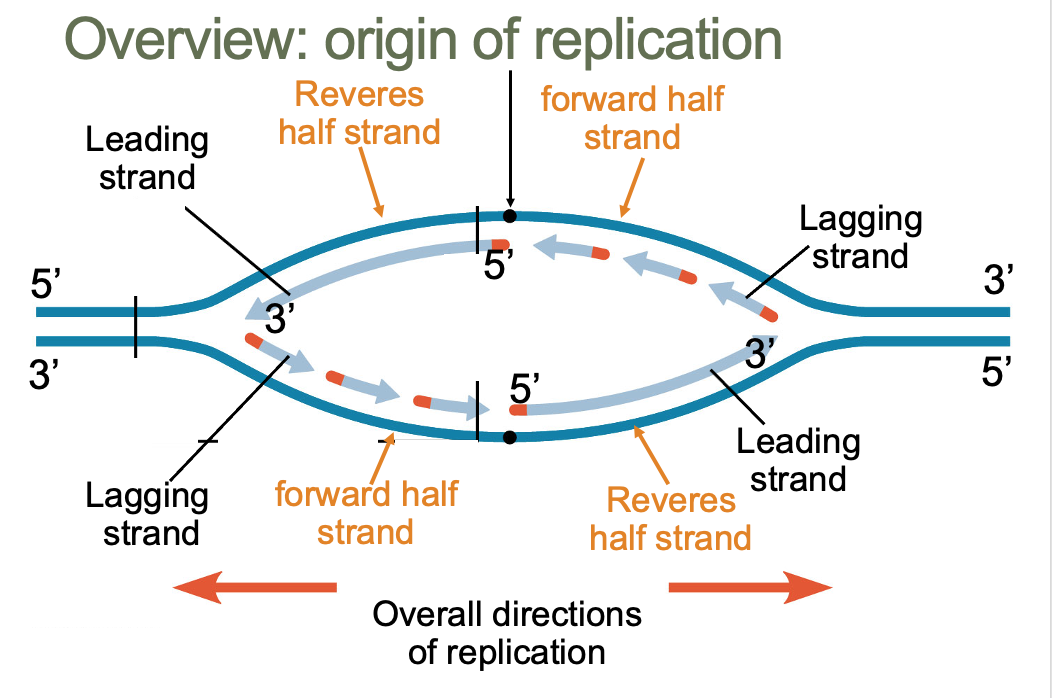
\includegraphics{./Images/img7.jpg}

One approach to finding \emph{oriC} would be to try to find some words
in the bacterial genome that indicate that region as where replication
starts. This could be done statistically, by finding unusually frequent
words (in the sense that it is more frequent in the DNA genome than in a
randomly generated sequence of the letters ``A'', ``G'', ``C'' and ``T''
of the same length) clumping together within short regions of the
genome. We are going to instead use an approach based on the content of
guanine and the content of cytosine in the genome, by using a sliding
window approach.

But why should the frequencies of G and C help settle this question?
This was hinted at in the lab. It turns out that replication generates
mutational anomalies due to the asymmetry of replication. This is
because DNA polymerase is \emph{unidirectional}, it can only transverse
DNA in the reverse direction (from 3' to 5'). This causes no problem for
the reverse half-strand, but the forward half-strand, which is unraveled
for replication from 5' to 3', can't be replicated from the start; it
must wait until there is enough space for the DNA polymerase (these
enzymes are huge biological machines, and need a fair amount of space
before binding) to bind a few nucleotides down the road and then be able
to replicate the short segment that was unraveled thus far in the
direction 3'-\textgreater{} 5'. These generates several phenomena in
DNA, such as the famous Okazaki fragments. What is relevant to us
though, is that, because of this, the forward half-strand spends much
more time single stranded than the reverse half-strand. And
single-stranded DNA has much higher mutation rates than double-stranded
DNA! \textbf{Specifically, C tends to mutate into T by a process called
deamination} \span.

The rate of deamination in single-stranded DNA is 100 times higher than
in double-stranded DNA. This creates mismatched pairs T-G which are then
corrected in the next replication into T-A pairs. It should be the case
then, that in the forward half-strand the C content should be low in
relation to the G content, and the opposite behavior in the reverse
half-strand (because the forward half-strand of the complementary strand
pairs with the reverse half-strand of the original strand). In
particular, \texttt{G\_content(genome)-C\_content(genome)}, for some
genome, should be smallest close to the \emph{oriC}, since \emph{oriC}
is the point that separates the beginning of the reverse half-strand and
the end of the forward half-strand.

3.1 With all of this said, let's analyze the most studied bacterial
genome: \emph{E. Coli}. \span

Put the \emph{E. coli}, \emph{Thermotoga petrophila} and
\emph{Sulfolobus solfataricus} in your working directory. The following
code loads all of these files into R.

\begin{Shaded}
\begin{Highlighting}[]
\NormalTok{e\_coli }\OtherTok{\textless{}{-}} \FunctionTok{read.fasta}\NormalTok{(}\StringTok{"Sequences/E. coli.fasta"}\NormalTok{)[[}\DecValTok{1}\NormalTok{]]}
\NormalTok{t\_petrophila }\OtherTok{\textless{}{-}} \FunctionTok{read.fasta}\NormalTok{(}\StringTok{"Sequences/Thermotoga petrophila.fasta"}\NormalTok{)[[}\DecValTok{1}\NormalTok{]]}
\NormalTok{s\_solfataricus }\OtherTok{\textless{}{-}} \FunctionTok{read.fasta}\NormalTok{(}\StringTok{"Sequences/Sulfolobus solfataricus.fasta"}\NormalTok{)[[}\DecValTok{1}\NormalTok{]]}
\end{Highlighting}
\end{Shaded}

(b) What we will do is try to find the point where the difference
between the G content and the C content achieves a minimum. For that,
write a function called \texttt{skew()} that receives as input a vector
of characters aka a DNA sequence (which in our case will be in fact a
whole bacterial genome) and a positive integer i and outputs the
difference between the G count and the C count from the first nucleotide
in the DNA sequence up to nucleotide number i (for i = 0, define the
skew to be 0). \span

\begin{Shaded}
\begin{Highlighting}[]
\NormalTok{skew }\OtherTok{\textless{}{-}} \ControlFlowTok{function}\NormalTok{(seq, i)\{}
\NormalTok{  skewVec }\OtherTok{\textless{}{-}} \FunctionTok{numeric}\NormalTok{(i)}
\NormalTok{  GC\_diff\_sofar }\OtherTok{\textless{}{-}} \DecValTok{0}
  
  \ControlFlowTok{for}\NormalTok{(ind }\ControlFlowTok{in} \DecValTok{1}\SpecialCharTok{:}\NormalTok{i)\{}
    \ControlFlowTok{if}\NormalTok{ (seq[ind] }\SpecialCharTok{==} \StringTok{"g"}\NormalTok{)\{}
\NormalTok{      skewVec[ind] }\OtherTok{\textless{}{-}}\NormalTok{ GC\_diff\_sofar }\SpecialCharTok{+} \DecValTok{1} 
\NormalTok{    \}}
    \ControlFlowTok{else} \ControlFlowTok{if}\NormalTok{ (seq[ind] }\SpecialCharTok{==} \StringTok{"c"}\NormalTok{)\{}
\NormalTok{      skewVec[ind] }\OtherTok{\textless{}{-}}\NormalTok{ GC\_diff\_sofar }\SpecialCharTok{{-}} \DecValTok{1} 
\NormalTok{    \}}
    \ControlFlowTok{else}\NormalTok{ \{}
\NormalTok{      skewVec[ind] }\OtherTok{\textless{}{-}}\NormalTok{ GC\_diff\_sofar}
\NormalTok{    \}}
\NormalTok{    GC\_diff\_sofar }\OtherTok{\textless{}{-}}\NormalTok{ skewVec[ind]}
\NormalTok{  \}}
  
  \FunctionTok{return}\NormalTok{(skewVec)}
\NormalTok{\}}

\NormalTok{exDNA}\OtherTok{\textless{}{-}} \FunctionTok{c}\NormalTok{(}\StringTok{"c"}\NormalTok{,}\StringTok{"t"}\NormalTok{,}\StringTok{"a"}\NormalTok{,}\StringTok{"t"}\NormalTok{,}\StringTok{"g"}\NormalTok{,}\StringTok{"g"}\NormalTok{,}\StringTok{"c"}\NormalTok{,}\StringTok{"g"}\NormalTok{,}\StringTok{"g"}\NormalTok{,}\StringTok{"g"}\NormalTok{,}\StringTok{"t"}\NormalTok{,}\StringTok{"a"}\NormalTok{)}
\FunctionTok{skew}\NormalTok{(exDNA, }\DecValTok{8}\NormalTok{)}
\end{Highlighting}
\end{Shaded}

\begin{verbatim}
## [1] -1 -1 -1 -1  0  1  0  1
\end{verbatim}

(c) Now, write a function called \texttt{skewDiagram()} that, given a
DNA sequence, outputs the skew diagram of the DNA sequence. A skew
diagram is a plot that has on the x axis positive integers (with x
ranging from 0 to the length of the DNA sequence), and on the y axis the
skew of the DNA sequence up to the index x. Hint: This is the first time
in this course you are going to face genomical analysis. One of its
challenges is that genomes are huge. Even a bacterial genome might be
non-trivial to a personal computer. Therefore, your implementation of
the algorithm might affect a lot the time you spend in this assignment.
Think carefully on how to implement your function. First of all, do not
recount G and C every time you need to compute some skew. Instead, find
a way of just updating previous skews. (**NOTE: to make this execute in
\textless\textless{} tens of minutes, plot
\texttt{skew{[}seq(1,\ length(skew),\ 10000){]}}
vs.~\texttt{seq(1,\ length(skew),\ 10000)}) Be sure to ask to your TA
for help if needed. Below is some pseudocode to get you started. Note
that the code is for both part b and c.\span 

\begin{Shaded}
\begin{Highlighting}[]
\CommentTok{\#PART C}
\CommentTok{\#second function to plot our skew vector}
\CommentTok{\#be sure to plot ONLY EVERY 10,000TH VALUE IN YOUR SKEW VECTOR }
  \CommentTok{\#hint: use seq()}
\NormalTok{skewdiagram }\OtherTok{\textless{}{-}} \ControlFlowTok{function}\NormalTok{(seq)\{}
\NormalTok{  skew }\OtherTok{\textless{}{-}} \FunctionTok{skew}\NormalTok{(seq, }\FunctionTok{length}\NormalTok{(seq))}
  \FunctionTok{plot}\NormalTok{(}\FunctionTok{seq}\NormalTok{(}\DecValTok{1}\NormalTok{, }\FunctionTok{length}\NormalTok{(skew), }\DecValTok{10000}\NormalTok{), skew[}\FunctionTok{seq}\NormalTok{(}\DecValTok{1}\NormalTok{, }\FunctionTok{length}\NormalTok{(skew), }\DecValTok{10000}\NormalTok{)], }\AttributeTok{xlab=}\StringTok{"Index in DNA Sequence"}\NormalTok{, }\AttributeTok{ylab=}\StringTok{"GC Skew"}\NormalTok{, }\AttributeTok{main=}\StringTok{"GC Skew Through DNA Sequence"}\NormalTok{)}
\NormalTok{\}}
\end{Highlighting}
\end{Shaded}

(d) Write a function \texttt{min\_skew} that, given a DNA sequence,
finds the i such that \texttt{skew(DNA,\ i)} is the minimum among
possible i. \span  

\begin{Shaded}
\begin{Highlighting}[]
\NormalTok{min\_skew }\OtherTok{\textless{}{-}} \ControlFlowTok{function}\NormalTok{(seq)\{}
\NormalTok{  skew }\OtherTok{\textless{}{-}} \FunctionTok{skew}\NormalTok{(seq, }\FunctionTok{length}\NormalTok{(seq))}
  \FunctionTok{return}\NormalTok{(}\FunctionTok{which.min}\NormalTok{(skew))}
\NormalTok{\}}
\end{Highlighting}
\end{Shaded}

(e) Now, use the functions you just wrote to analyze the genome of
\emph{E. coli}. Given the skew diagram of \emph{E. coli}, report
\textbf{and justify} where you expect \emph{oriC} to be located in the
\emph{E. coli} genome (notice that the minimum may differ from
\emph{oriC} due to random fluctuations in the G or C frequencies, hence,
you should really indicate a short region rather than a point). (Hint:
your suggested region should be a span 500 to 1000 nucleotides long)
\span 

\begin{Shaded}
\begin{Highlighting}[]
\FunctionTok{skewdiagram}\NormalTok{(e\_coli)}
\end{Highlighting}
\end{Shaded}

\includegraphics{CompAsn3_BIOS11141_files/figure-latex/unnamed-chunk-22-1.pdf}

\begin{Shaded}
\begin{Highlighting}[]
\FunctionTok{min\_skew}\NormalTok{(e\_coli)}
\end{Highlighting}
\end{Shaded}

\begin{verbatim}
## [1] 3925597
\end{verbatim}

{ I expect the oriC to be around the 3,925,000 - 3,926,000 base. This is
around the minimum point of the GC skew. GC skew should be minimized at
the Ori because deamination of the complementary strand reduces G
content left of the Ori and the G content should be higher on the right
side. }

3.2 Now, load the genome of \emph{Thermotoga petrophila} and plot its
skew diagram. How is this different from that of \emph{E. coli}? Where
would you expect the \emph{oriC} of \emph{Thermotoga petrophila} to be?
\span

\begin{Shaded}
\begin{Highlighting}[]
\FunctionTok{skewdiagram}\NormalTok{(t\_petrophila)}
\end{Highlighting}
\end{Shaded}

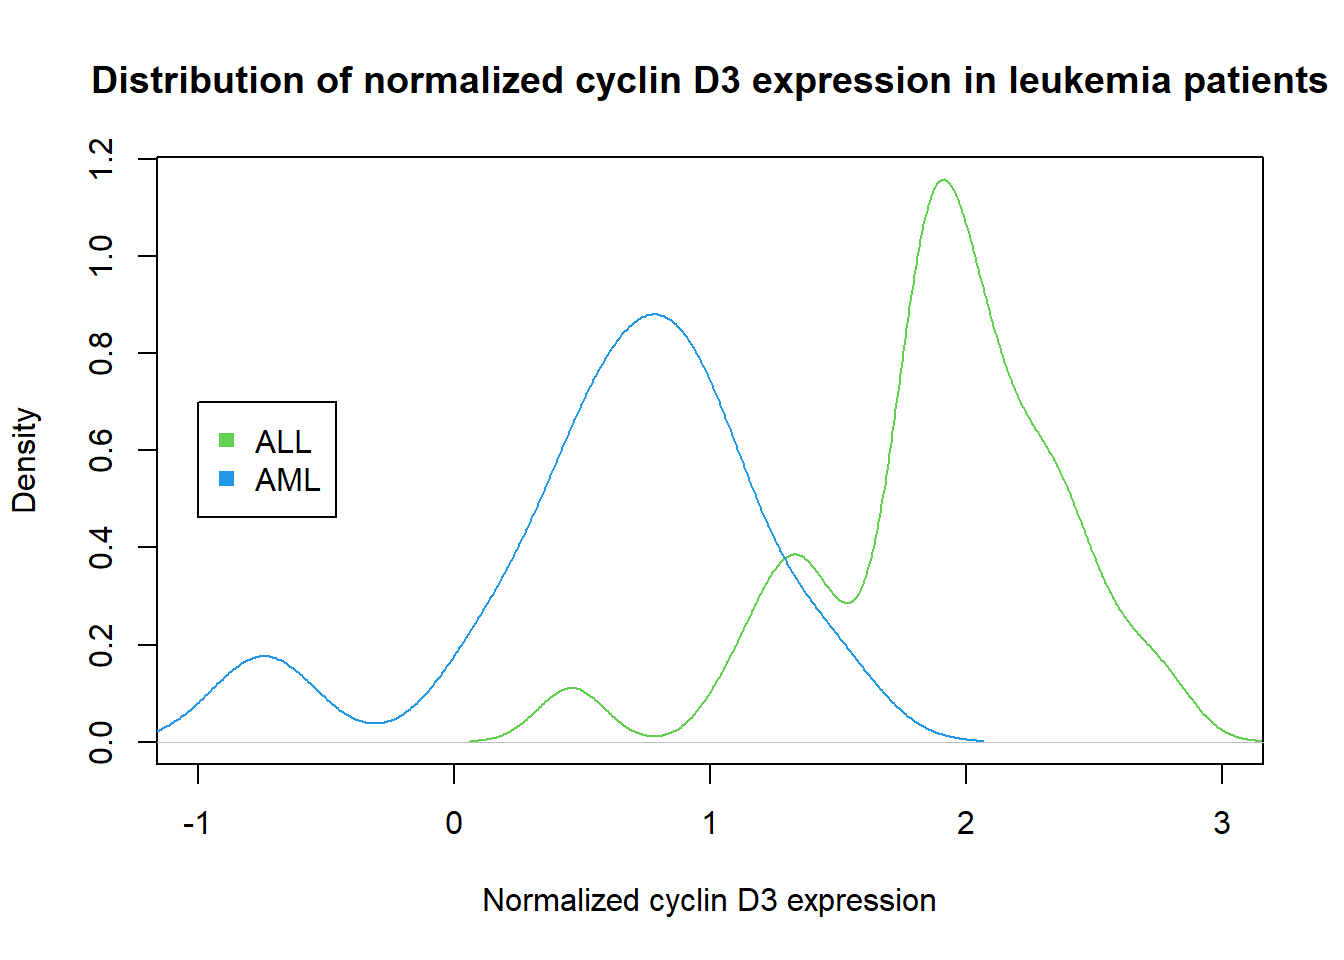
\includegraphics{CompAsn3_BIOS11141_files/figure-latex/unnamed-chunk-24-1.pdf}

\begin{Shaded}
\begin{Highlighting}[]
\FunctionTok{min\_skew}\NormalTok{(t\_petrophila)}
\end{Highlighting}
\end{Shaded}

\begin{verbatim}
## [1] 787199
\end{verbatim}

{ This is different from the skew diagram of E. coli in that it has
multiple local minima rather than in the E. coli genome where there was
one clear minimum. I would expect the oriC to be at the global minimum
of the GC skew which is around the 787,000-788,000 base. }

3.3 Load the genome of the archea \emph{Sulfolobus solfataricus} and
plot its skew diagram. We've seen that the minimum skew provides a guess
for the \emph{oriC} of bacterial genome. Notice though, that we were
focusing on global minima. You can see on the skew diagram of
\emph{Sulfolobus solfataricus} that there are three clear valleys were
you can identify local minima. What might this indicate? Try to find
published experimental evidence that proves your hypothesis. \span

\begin{Shaded}
\begin{Highlighting}[]
\FunctionTok{skewdiagram}\NormalTok{(s\_solfataricus)}
\end{Highlighting}
\end{Shaded}

\includegraphics{CompAsn3_BIOS11141_files/figure-latex/unnamed-chunk-26-1.pdf}

\begin{Shaded}
\begin{Highlighting}[]
\FunctionTok{min\_skew}\NormalTok{(s\_solfataricus)}
\end{Highlighting}
\end{Shaded}

\begin{verbatim}
## [1] 749375
\end{verbatim}

{ The presence of multiple local minima could indicate that there are
multiple origins of replication. This theory seems to be supported by
\href{https://www-ncbi-nlm-nih-gov.proxy.uchicago.edu/pmc/articles/PMC7525243/}{this
article} }

\end{document}
